\documentclass{standalone}
\usepackage{xcolor}
\usepackage{verbatim}
\usepackage[T1]{fontenc}
\usepackage{graphics}
\usepackage{hyperref}
\newcommand{\code}[1]{\texttt{#1}}
\newcommand{\R}{R}
\newcommand{\pkg}[1]{#1}
\newcommand{\CRANpkg}[1]{\pkg{#1}}%
\newcommand{\BIOpkg}[1]{\pkg{#1}}
\usepackage{amsmath,amssymb,array}
\usepackage{booktabs}
\usepackage{subcaption}
\usepackage{multirow}
\usepackage{tikz}
\usetikzlibrary{automata,arrows,positioning,calc}

\begin{document}
\nopagecolor
	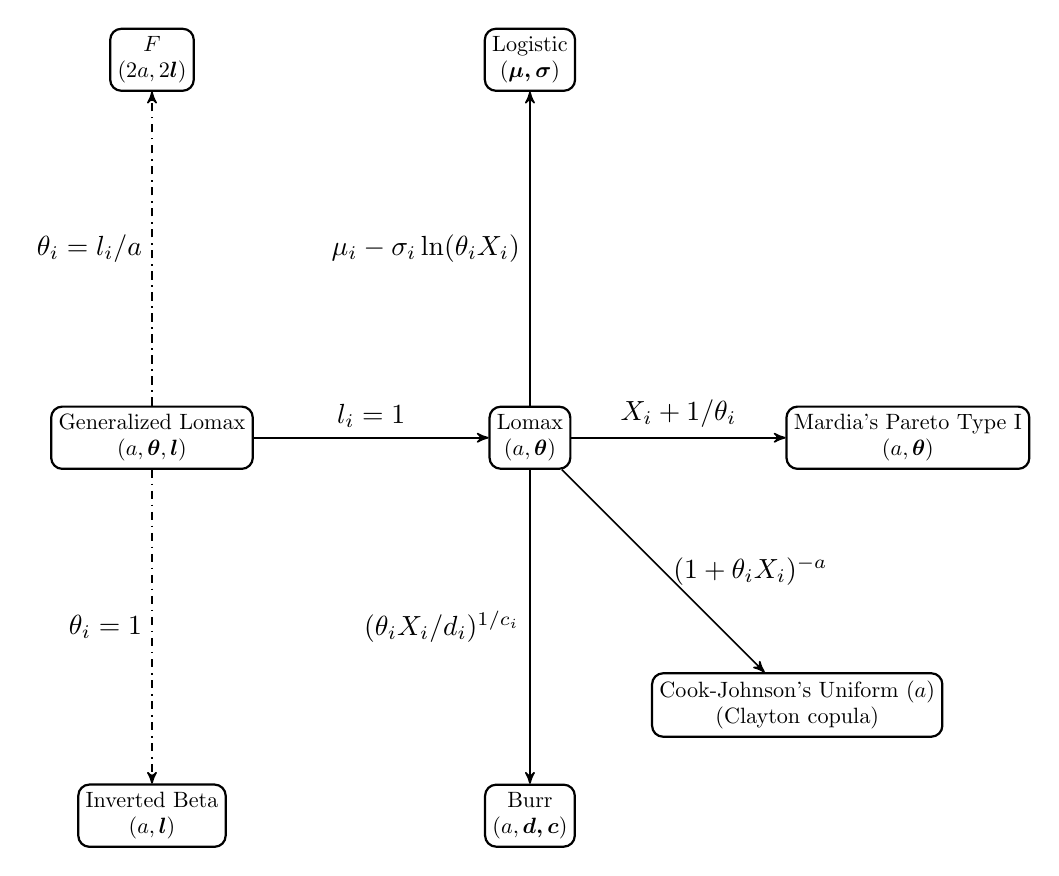
\begin{tikzpicture}[->, >=stealth', auto, semithick, node distance=6cm]
	\tikzstyle{every state}=[rectangle, fill=white,draw=black,thick,text=black,scale=0.8,align=center,rounded corners]
	\node[state]   (GLomax)      {Generalized Lomax \\ $(a, \boldsymbol{\theta}, \boldsymbol{l})$};
	\node[state]    (Lomax)[right of=GLomax]   {Lomax \\ $(a, \boldsymbol{\theta})$};
	\node[state]    (MPareto)[right of=Lomax]   {Mardia's Pareto Type I \\ $(a, \boldsymbol{\theta})$};
	\node[state]    (Logistic)[above of=Lomax]   {Logistic \\ $(\boldsymbol{\mu, \sigma})$};
	\node[state]    (Burr)[below of=Lomax]   {Burr \\ $(a, \boldsymbol{d, c})$};
	\node[state]    (Uniform)[below right of=Lomax]   {Cook-Johnson's Uniform $(a)$ \\ (Clayton copula) };
	\node[state]    (F)[above of=GLomax]   {$F$ \\ $(2a, 2\boldsymbol{l})$ };
	\node[state]    (InvBeta)[below of=GLomax]   {Inverted Beta \\ $(a, \boldsymbol{l})$};
	\draw (GLomax) -- (Lomax) node [midway, above, sloped] (TextNode) {$l_i = 1$};
	\draw (Lomax) -- (MPareto) node [midway, above, sloped] (TextNode) {$X_i + 1/\theta_i$};
	\draw (Lomax) -- (Logistic) node [midway, left, sloped=90] (TextNode) {$\mu_i-\sigma_i\ln(\theta_iX_i)$};
	\draw (Lomax) -- (Burr) node [midway, left, sloped=90] (TextNode) {$(\theta_iX_i/d_i)^{1/c_i}$};
	\draw (Lomax) -- (Uniform) node [midway, right, sloped=90] (TextNode) {$(1+\theta_iX_i)^{-a}$};
	\draw [dash dot] (GLomax) -- (F) node [midway, left, sloped=90] (TextNode) {$\theta_i=l_i/a$};
	\draw [dash dot] (GLomax) -- (InvBeta) node [midway, left, sloped=90] (TextNode) {$\theta_i=1$};
	\end{tikzpicture}
\end{document}
